%!TEX root = ../thesis.tex
%*******************************************************************************
%****************************** Second Chapter *********************************
%*******************************************************************************

\chapter{Quantifying received dose errors introduced by modelling approximations in reinforced concrete shielding}
\label{chap:homogenisation}

\ifpdf
    \graphicspath{{Chapter2/Figs/Raster/}{Chapter2/Figs/PDF/}{Chapter2/Figs/}}
\else
    \graphicspath{{Chapter2/Figs/Vector/}{Chapter2/Figs/}}
\fi

% ITER report is robust and actually quite well written, use as base
% Check with Roddy I can use material from this report
% Need some introductory material on spatial homogenisation:
%     Raoul's report?
%     Wider literature
% Additional figures which might be nice:
%     Nice SDDR photon ratio
%     Interpolated (time, E, ratio) heatmap

\section{Outline}
This chapter looks to determine the impact of a nuclear analysis modelling approximation known as spatial homogensation--where complex geometries of differing materials are combined to form a homogeneous volume with a new material mixture. An introduction to radiation shielding is given. Then, undertaking a study for and of relevance to ITER, the effect of spatial homogenisation on the attenuation properties of reinforced concrete walls is investigated. A comparative method is described and subsequently the impact of spatial homogenisation on the shut-down dose rate to workers is also analysed. The effects of spatial homogenisation have at most a 22\% underestimate for on-load doses in the cases modelled here. The shut-down dose rates are slightly overestimated by spatial homogenisation.

%INTRODUCTION
\section{Introduction}
The ITER nuclear fusion experiment will begin DT operation in the 2030s. At 500MW fusion power the source rate of 14.1MeV neutrons will approximately $1.8\times10^{20}$ s\textsuperscript{-1}. For comparison, JET's maximum source rate to date is 30 times less. But the real difference is in the fluence. JET's lifetime neutron budget is now set at $2\times10^{21}$ \cite{Lobel2008}, or 10 seconds of operation for ITER-DT. The ITER life-time budget is approximately $3\times10^{27}$ neutrons.

Designing a complex device such as a superconducting tokamak to operate in this radiation environment is a particularly challenging aspect of the ITER project. Care must be taken both to shield sensitive components like semiconductor devices from Single Event Effects (SEE) and to prevent excessive nuclear heating in large systems like the superconducting coils. The high flux and fluence of high energy neutrons means activation in areas like the Neutral Beam (NB) cells and in the Tokamak Cooling Water System (TCWS) will be significant. And of course, gamma from these activated components, and the prompt radiation of a thermonuclear plasma must be shielded against to protect the workforce operating and maintaining the plant.

Quantifying the absorbed dose to radiation sensitive components, or the equivalent dose to personnel requires crafting a computer model of the problem and typically making a series of assumptions and simplifications in the process. For reinforced concrete radiation shields, this often entails either homogenising the rebar with the concrete, or even neglecting the presence of rebar entirely. This process introduces systematic error into the reported solution of the problem. So, in addition to uncertainties from cross-section, secondary particle and decay data as explored in chapter~\ref{chap:tmc}, modelling approximations play a role in thickening the fog of misunderstanding. 

\subsection{Radiation shielding}
A fusion reactor harbours many different radiation fields. A variety of particles, across the energy spectrum, are present at one time or another. In order to preserve biological life and to extend the operable life of components, radiation shielding is employed to attenuate radiation fields, reducing their intensity by many orders of magnitude.

\subsubsection{Radiation fields}
The radiation fields of principal interest for shielding in fusion systems are the neutron and photon fields both during and after operation of the device.

\begin{itemize}
  \item Prompt neutron--During a plasma shot, fusion neutrons will be emitted from the plasma at around 14.1 and 2.5 MeV for DT and DD reactions respectively. These neutrons propagate out of the plasma unheeded due to the very low plasma density. The uncharged particles travel in straight lines until they encounter a nucleus in the surrounding material. For a fusion reactor this will be the first wall, divertor or initial layers of the blanket. The neutrons then scatter elastic and inelastically off nuclei, losing energy in the process by transferring it to the bombarded nuclei. Eventually the neutrons reduce in energy to the $1/v$ region of nuclear interaction, where lower energies (velocities, $v$) are favoured as the time for neutron-nuclei interaction is increased. At these low energies, reactions like radiative capture become very likely and neutron fluxes decrease through absorption.
  \item Prompt photon--While a fusion reactor is running, a large amount of Bremsstrahlung radiation will be emitted from the plasma at energies in the keV range and $\gamma$ photons at MeV energies can be emitted by certain hydrogenous nuclear reactions. However, other radiation will be generated by the interaction of neutrons with surrounding matter. As the neutrons slow down their inelastic collisions excite nuclei which return to a ground state by emission of an energetic photon. This process generates an intense photon field.
  \item Shut-down photon--After cessation of plasma operations, there will still be intense radiation fields within and around a tokamak. The fusion neutrons will have activated and transmuted nuclei through reactions such as radiative capture. Many of the reconfigured nuclei will not be stable and so will decay through various emission mechanisms to a stable ground state. This often involves a chain of $\gamma$ and other emissions.
  \item Shut-down neutron--Despite the lack of fusion neutrons after the reactor has turned off, a neutron field still persists. Reactions such as photofission of actinide contaminants, $^{2}$H($\gamma$,n)$^{1}$H in cooling water \cite{Kodeli1995} and $^{9}$Be($\gamma$,n$\alpha$)$^{4}$He in the first-wall \cite{Davis2010} will generate neutrons.
\end{itemize}

\subsubsection{Shielding design}
Shielding for a fusion system will have to attenuate the above fields to an acceptable level for the safety of humans and the wider environment, as well as any equipment which is sensitive to radiation. The basic principal for shielding photons is to use Compton scattering (see chapter~\ref{chap:introduction}, section~\ref{subsubsec:compton}) off electrons to reduce the photon energy until they are absorbed. Therefore the higher the electron density, the greater the $\gamma$ shielding properties of a material. For this reason, high-Z materials such as heavy metals like steel, lead and tungsten are frequently used. Shielding for neutrons is similar in approach, moderating and then absorbing, although different materials are suitable. For moderation low-mass nuclides are best, to maximise the energy transfer with each collision (see equation~\ref{eq:alpha} in section~\ref{subsubsec:elastic}, chapter~\ref{chap:introduction}). The best nuclide is $^{1}$H, so any hydrogenous substance such as water provides an effective neutron moderator. Once moderated, absorption is best achieved by nuclides with a large radiative capture cross-section. There are many considerations in designing a long-lived, effective radiation shield, especially for high-flux operation. Any shield design will have to balance parameters such as cost, weight, volume, radiation damage, self-activation and nuclear heating. A much more complete discussion of radiation shielding design can be found in \cite{Price1959}.

\section{Method}
The modelling simplification under investigation is that of spatial homogenisation and how it affects doses to workers, whether prompt or delayed. It is theorised that any errors incurred by this modelling approximation will be functions of geometry and material composition. For each set of variables interrogated, at least two simulations will be performed. One will have a high-fidelity model of the real-world problem geometry with reinforcing bar and stirrup rods faithfully reproduced. The other will smear the rebar across the concrete, homogenising the two materials into one with a density equal to the mass weighted sum of the concrete and steel constituents. 

Simulations employing realistic ITER source particle distributions will tally transmitted or `leakage' fluence at the rear of the shielding walls in both cases. This permits comparison between the modelling approximation and the higher-fidelity simulation.

The implications of spatial homogenisation prove to be different for on-load and shut-down (activated) dose rates. It is helpful to consider them seperately. The following two sections detail the methods for determining these two dose rates.

\subsection{Prompt neutron \& gamma radiation}
Determining the dose to personnel beyond a wall requires knowledge of the radiation fluxes there. The on-load gamma flux $\phi_{\gamma}(x,y,z,E,t)$ and neutron flux, $\phi_{n}(x,y,z,E)$, can be computed with Monte Carlo techniques, spawning neutrons from a prerecorded source distribution, $P(x,y,z,E,\Omega)$ at a particular point with a given energy and angle. These particles may propagate through the wall, scattering, being absorbed, exciting nuclei (which later relax through radiative emission) and perhaps leaking out of the back of the shield wall. Tallying this leakage flux of neutrons and photons is the main task of calculating a dose due to radiation.

\subsubsection{Model geometry}
The heterogeneous, realistic wall is constructed of a large concrete block, with two meshes of rebar, one buried below each face. The distance from wall exterior to rebar is known as the cover depth. Connecting the two meshes are a small number of narrow gauge `stirrup' bars. The homogeneous model is the same external dimensions and total mass as the heterogeneous one, but without an internal steel structure and with homogenised materials.

A Python program has been written to take wall thickness, cover depth and other parameters as input variables to construct a corresponding MCNP model. This model utilises lattices to construct the repeated features of the reinforced concrete wall. The concrete block dimensions are $(x, y, z) = (10, y, 10)$ where $y$ is the wall thickness. Embedded within the block are the major two meshes of steel reinforcement. These meshes are always constructed with 200mm spaced rebar extendeding in both the x and z directions \cite{Perez2014}. The meshes are buried a small cover depth from the two $y$-perpendicular surfaces of the wall. Tying the two meshes together are some thinner `stirrup' bars extending in the y direction, with $\approx 4m^{-2}$ of wall face \cite{Perez2014}. A particular level of reinforcement may be referred to as 16HB200, i.e. 16mm diameter rebar, at 200mm spacing.

Simulations were run for the following wall thicknesses: 30, 50, 80, 120 \& 210 cm. For each case, the fraction of total wall mass as steel was kept constant at 4.45\%. This was achieved by increasing the rebar diameter, noting the relationship shown in equation~\ref{eq:rebar}. 

\begin{equation}
  \label{eq:rebar}
  \frac{d^{2}_{r}}{t_{w}} \propto f_{s}
\end{equation}

That is, the rebar diameter, $d_{r}$ squared divided by the wall thickness, $t_{w}$ is proportional to the steel fraction, $f_{s}$. The value of 4.45\% was chosen as this is a typical value computed from the description of reinforcement and dimensions in \cite{Perez2014}. 

Material compositions, wall widths, rebar arrangements and steel fractions have been determined from ITER drawings and specifications for concrete walls in the tokamak building. The work has been conducted with a moderated ITER DT fusion neutron source spectrum. The results should give a good idea of the implications of the homogeneous modelling approximation at ITER but also more generally given the standard civil engineering design of the reinforced concrete walls.

% column span figure
\begin{figure}[h]
  \figuretitle{Homogenising reinforced concrete}
  \includegraphics[width=\textwidth]{wall_diagram}
  \caption{The two modelling approaches considered in this investigation. a) Heterogeneous, where the steel reinforcing bar and stirrups are explicitly modelled. b) Homogeneous, where the mass of rebar is 'smeared' through the concrete. The new homogenised material has a greater density than plain concrete, conserving mass.}
  \label{fig:wall_diagram}
\end{figure}

\subsubsection{Materials}
Although much of the investigation will be by comparing values for homogeneous and heterogeneous responses, it is still important to supply the most accurate input information possible for the simulations. All the compositions that follow were mixed using the PyNE python package \cite{Pyne18} employing natural abundance for isotopic distributions.

\paragraph{Concrete}
The density of concrete used is 2.2g cm\textsuperscript{-3} \cite{Jakhar16}. The composition is shown in table~\ref{tab:concrete} in appendix~\ref{app:materials}. 

\paragraph{Steel}
The density of steel used for rebar is 7.85g cm\textsuperscript{-3} \cite{BSsteel05}. The steel minor constituents Cu, Mn, Cr, Mo, V and Ni are not specified in \cite{BSsteel05} however the CEV (Carbon Equivalent Value) is given, a figure for quantitatively comparing the `weldability' of steels. The CEV formula was used to determine likely \% fractions of the aforementioned elements, giving a material composition as shown in table~\ref{tab:steel} in appendix~\ref{app:materials}.

\subsubsection{Radiation sources}
The effect of spatial homogenisation is considered for both neutron and photon radiation, hence likely distributions are required for both particle types.

No particle direction information was available, so it was assumed that all particles are born travelling perpendicular to the radiation shield. It was reasoned that this is a conservative assumption, liable to increase the discrepancy between heterogeneous and homogeneous approaches as the heterogeneous model has features (the stirrup bars) which are aligned with this initial particle direction.

% column span figure
\begin{figure}[H]
  \figuretitle{ICRP74 flux to dose factors}
  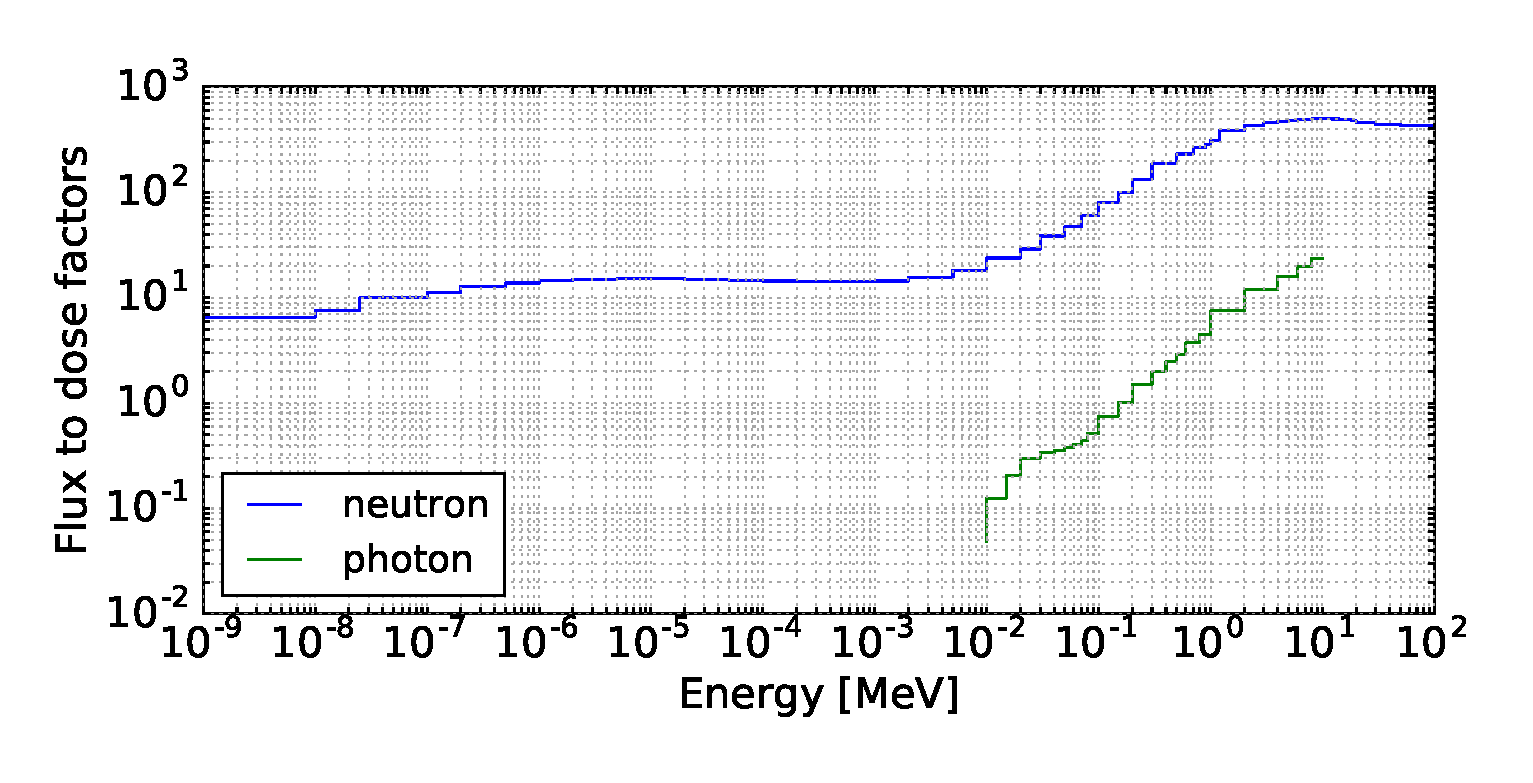
\includegraphics[width=\textwidth]{icrp74}
  \caption{The flux to dose conversion factors for neutron and photon exposure.}
  \label{fig:icrp74}
\end{figure}

The effective dose to humans is a function of the energy and type of radiation. It takes into account the varying susceptibilities of different tissues in the human body. For radiation protection, this is the typical figure quoted when specifying a dose rate. Where required, translation from fluence or flux to dosea or dose-rate respectively is by functions as shown in figure \ref{fig:icrp74}.

\paragraph{Neutron}
The neutron source spectrum was obtained in previous work by \citeauthor{Jakhar16} and is shown below as \ref{fig:src_spectra}. The location tallied for this particle spectrum was behind a ITER neutral beam assembly, of neutrons incident upon the shield wall behind. In the ITER plant this area will receive an elevated flux over other areas of the bioshield due to the penetrations from neutral beam injectors into the plasma chamber. The neutron spectrum was provided in the 175 VITAMIN-J group structure. Unfortunately this group structure provides very little information about the fine structure of the thermal neutron distribution below 0.1 eV. This is a deficiency in this study as the source spectrum is heavily thermalised. For the radiation transport simulations, no neutron source rates or wall loadings were specified. Instead, results were reported per source neutron. Many of the results later presented are ratios of the same quantity and hence unitless. 

% column span figure
\begin{figure}[H]
  \figuretitle{Neutron source spectrum}
  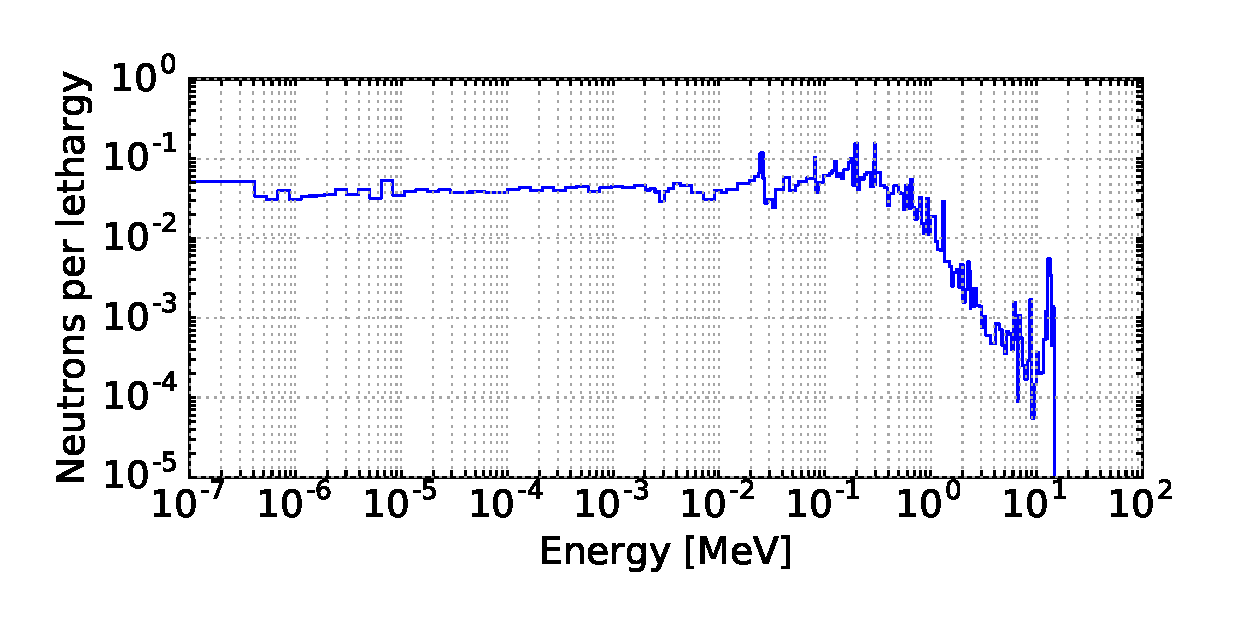
\includegraphics[width=\textwidth]{src_spectra}
  \caption{Neutron spectra for incident radiation. This spectra was tallied at back of the ITER Neutral Beam assembly.}
  \label{fig:src_spectra}
\end{figure}

\paragraph{Photon}
The Tokamak Cooling Water System (TCWS) will move large quantities of water through an intense neutron flux during ITER's operation. This water leaves the tokamak through a network of penetrations and pipes in the surrounding facility. The water is activated mainly by the following reactions: \textsuperscript{16}O(n,p)\textsuperscript{16}N and \textsuperscript{17}O(n,p)\textsuperscript{17}N. These nitrogen isotopes rapidly decay as shown in table~\ref{tab:nitrogen_decay}.

\begin{table}[H]
  \centering
  \begin{tabu} to \textwidth {X[3] X X X[5]}
    \toprule
    Activation product  & t$_{\frac{1}{2}}$(s)  & Decay mode  & Energy (MeV) [branching ratio \%] \\
    \midrule
    \textsuperscript{16}N & 7.13 & $\gamma$              & 6.129 [67], 7.115 [5] \\
    \textsuperscript{17}N & 4.14 & $\beta \rightarrow n$ & 0.383 [35], 1.171 [53] \\
    \bottomrule
  \end{tabu}
  \caption{The type, energy and likelihood of decay from activated N isotopes in the ITER water cooling system.}
  \label{tab:nitrogen_decay}
\end{table}

The gamma decay of \textsuperscript{16}N is utilised as a source for several of the simulations presented in section~\ref{subsec:prompt}.

\subsubsection{Computation}
\label{subsubsec:rad_tran_comp}
The nuclear data employed was the continuous energy Joint Evaluated Fission and Fusion file 3.2 (JEFF3.2) for neutron transport and MCPLIB84 for photon transport. EAF2010 data was used at ITER Organisation's request for activation calculations. Radiation transport was conducted with MCNP6v1.0

The MCNP relative error, $R = \frac{\sigma_{s}}{\mu_{s}}$ which is the ratio of sample standard deviation to sample mean was kept to below 0.1 for all energy bins and mesh voxels where possible. However, the wall is a shield and heavily attenuating of source particles. For a 50cm thickness of concrete, the neutron attenuation is approximately 7 orders of magnitude. Therefore in order to converge the spectrum and solve the problem a significant number of histories must be run. 

Converging results on a coarse energy grid or `group structure' requires fewer source particles for a given $R$, but having fewer energy bins means the spectrum will be correspondingly poorly resolved, with large steps in flux across the energy domain. Initial simulations using VITAMIN-J 175 group structure did a good job of resolving the spectrum from 1 eV up to the fusion peak at 14MeV, however they completely fail to represent the fine structure of the thermal spectrum. This is demonstrated in figure~\ref{fig:neutron_group_comparison}. The two lowest bins are $[10^{-5},10^{-1})$ eV and $[10^{-1},4.1\times10^{-1})$ eV. Despite the lack of thermal energy resolution, VITAMIN-J extends to very low energies. This means that neutrons scored at thermal energies contribute equally across four orders of magnitude in the lowest bin. When a spectrum such as this is sampled later, for an activation calculation, say, fictitious neutrons at $10^{-5}$ and $10^{-4}$ eV are produced and will skew results for problems where reactions in the 1/E region are significant, potentially drastically overestimating reaction rates. 

\begin{figure}[H]
  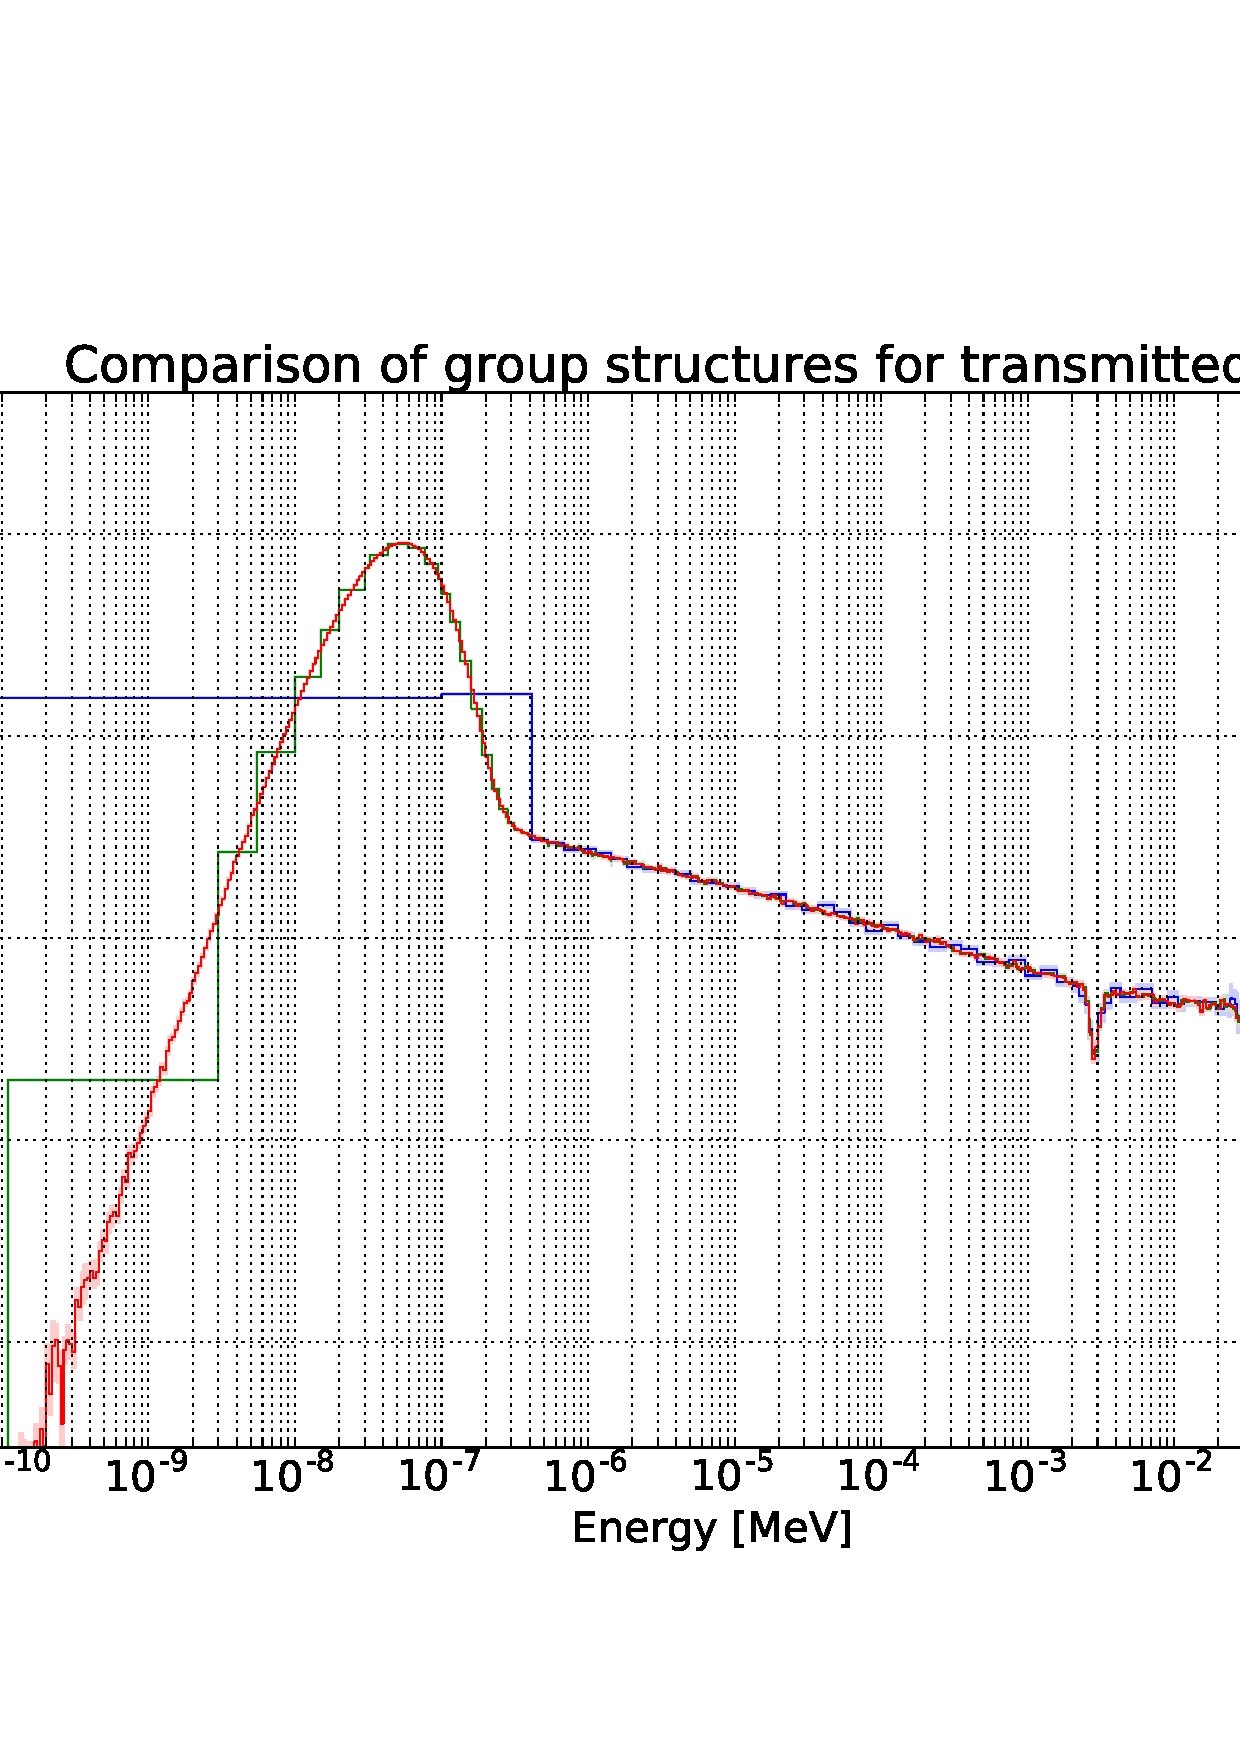
\includegraphics[width=\textwidth]{shield_flux_by_group.png}
  \caption{This figure shows the same transmitted flux, as simulated by MCNP, binned in a variety of group structures. While the region down to approximately 1 eV is resolved broadly similarly, the VITAMIN-J 175 group structure has insufficient bins to resolve a Maxwellian distribution of thermal neutrons in the low-energy region.}
  \label{fig:neutron_group_comparison}
\end{figure}

The ideal group structure should contain enough bins in the low energy region to approximate a thermal distribution. However, as previously stated, all bins should converge to have a relative error of less than 0.1 as proof of convergence. For this particular problem, convergence is most difficult for the high energy region, as these particles are relatively rare. Hence, many fine bins in the high energy region will necessitate significantly longer run times. For the work presented here, the 315 neutron group structure was selected as a compromise between speed and fidelity.

%\begin{equation}
%\lambda_{D(e)}=\sqrt{ \frac{ \varepsilon_0 k_B T_{(e)}}{e^2 n_\infty}}
%\end{equation}

\subsection{Shut Down Dose Rate (SDDR)}
The calculation of $\phi_{\gamma}(x,y,z,E,t)$ where $t$ is some time after cessation of plasma operation comprises three main steps:
\begin{enumerate}
  \item Neutron transport---as previously, compute the neutron flux during plasma operation, $\phi_{n}(x,y,z,E)$, recording the neutron flux binned by energy over a spatial mesh. Finer meshes will converge on true behaviour, with coarse meshes over or under-estimating fluxes depending on local geometry and flux gradients \footnote{Using a mesh which conforms to the geometry, such as an unstructured mesh, has been shown to give significant improvements, especially for small features \cite{Eade2015}.}.
  \item Activation---determine the appropriate irradiation scenario, then activate and transmutate the materials present in the problem geometry. This involves assembling a system of differential equations, Bateman equations, to track the inventory of all the nuclides present. One can numerically solving this system for a series of timesteps using codes such as FISPACT-II \cite{sublet2017a}. The resulting nuclides and their abundances can be paired with decay data to generate a decay photon source on the original mesh. 
  \item Photon transport---using the distributed decay gamma source produced by step 2), conduct a radiation transport run to determine the photon flux, $\phi_{\gamma}(x,y,z,E,t)$, converting to effective dose as required.
\end{enumerate}

\subsubsection{Model geometry}
The shut-down dose rate is calculated for the following scenario: it assumes a worker is inside the bioshield at ITER during a shutdown, stood 30cm from the inner surface of a 150cm thick wall with a steel mass fraction of 4.5\% the total wall mass. Reinforcing bar forms a mesh of squares 20cm in width and height at the front and back of the wall, 5cm from the surfaces. 

\subsubsection{Materials}
For analysis of the SDDR, where small impurities can have large contributions to the dose rate, the steel composition was refined \cite{Barabash16}. ITER limits for Co and Ni were imposed, 0.01\%wt and 0.05\%wt respectively. The resulting composition for steel is shown as table~\ref{tab:sddr_steel} in appendix~\ref{app:materials}.

\subsubsection{Computation}
As for before, radiation transport was conducted with MCNP6 v1.0. Neutron spectra were tallied on a mesh in the shield models. These spectra were used as input to the MCR2S activation linker code \cite{Davis2010a}. This program uses these spectra and a corresponding irradiation scenario to compute material changes within the meshed model. These new materials and decay information can be used to generate a photon source from the activated nuclides. The final steps in the calculation are to perform photon transport calculations from the activated wall to a target. The generation of photon sources and transport of emitted $\gamma$-rays must be computed for each decay time step of interest.

The irradiation scenario employed for the activation step was ITER's SA-2 \cite{Loughlin09}, which approximates the ITER DT experimental programme total fluence and explicitly includes the final, end-of-life pulses for accurate estimation of short-lived nuclides.

As noted in section~\ref{subsubsec:rad_tran_comp}, the choice of energy group structure can be important for the accuracy of calculations. When a pre-sampled neutron flux is later sampled to calculate a SDDR dose, the 175 group structure introduced a 20\% increase in dose rate for steel at all time steps, and approximately the same increase for concrete until days after irradiation, when the discrepancy between 175 and 315 falls to zero.

The dominant contributors to dose rate in steel all originate through (n,$\gamma$) and as such are not threshold reactions, instead observing 1/E behaviour at low energies. Whilst the dominant contributor to dose rate in concrete is initially \textsuperscript{24}Na formed though \textsuperscript{23}Na(n,$\gamma$)\textsuperscript{24}Na, it decays with t$_{\frac{1}{2}}=15$h before the dominant nuclide becomes \textsuperscript{39}Ar, which is produced via \textsuperscript{39}K(n,p)\textsuperscript{39}Ar. The (n,p) reaction is threshold, i.e. not effected by the low energy inaccuracy introduced by binning in 175. Therefore after a few days, the SDDR discrepancy between groups reduces to zero.

Further enquiry into the optimum energy group structures for activation calculations is presented as chapter~\ref{chap:group_structure}.

%%%%%%%%%%%%%%%%%%%%%%%%%%
% RESULTS AND DISCUSSION %
%%%%%%%%%%%%%%%%%%%%%%%%%%
\section{Results \& discussion}
This section details the effect of spatial homogenisation on fluence and dose received by workers in several circumstances. First, on-load radiation: neutrons originating from the plasma and multiplication reactions within the reactor and photons emitted from neutron induced reactions such as inelastic scattering and activation of nitrogen in water. Subsequently, a case is investigated where neutrons are transported through the shielding wall, activate it and then the resulting gamma-rays transported, this time tallied on the inner side of the wall--estimating the dose received by workers performing a maintenance action between plasma shots.

\subsection{Transmission of prompt radiation}
\label{subsec:prompt}
As neutrons from the ITER plasma are incident upon the shielding wall, they advance through the material. Nuclides from steel and concrete materials scatter the neutrons, moderating their energy down. Figure~\ref{fig:mfp} shows the neutrons have a mean free path of approximately 2cm in concrete, and most will scatter multiple times in the material--although the path length distribution is relatively broad, and some may travel 10cm or more without interaction. As the energy decreases, the likelihood of capture increases. Indeed, most neutrons are eventually absorbed, although a small fraction of the source particles propagate all the way through the shield and an even smaller proportion without any interactions at all--the DD and DT peaks visible in figure~\ref{fig:trans_neutron_spec}. 

\begin{figure}[H]
  \centering
  \figuretitle{Neutron path length in concrete}
  \includegraphics[width=0.7\textwidth]{mfp}
  \caption{The path lengths of neutrons in pure concrete are shown as a histogram. There is a wide distribution with a mean of approximately 2cm. This figure was compiled from MCNP ptrac data.}
  \label{fig:mfp}
\end{figure}

The transmitted, or `leakage' neutron spectra for a thick (2.1m) concrete wall is shown below as figure~\ref{fig:trans_neutron_spec}. Note the DT and prominent DD reaction peaks at 14.1 and 2.5 MeV respectively. Other features are the flat slowing-down region with a few flux depressions and the significant thermal Maxwellian distribution. The flux has been severely reduced by its interaction with the wall, decreasing from the source by an order of magnitude each 20cm traversed. The most prominent difference between the heterogeneous and homogeneous models is in the thermal region. 

\begin{figure}[H]
  \centering
  \figuretitle{Transmitted neutron spectra}
  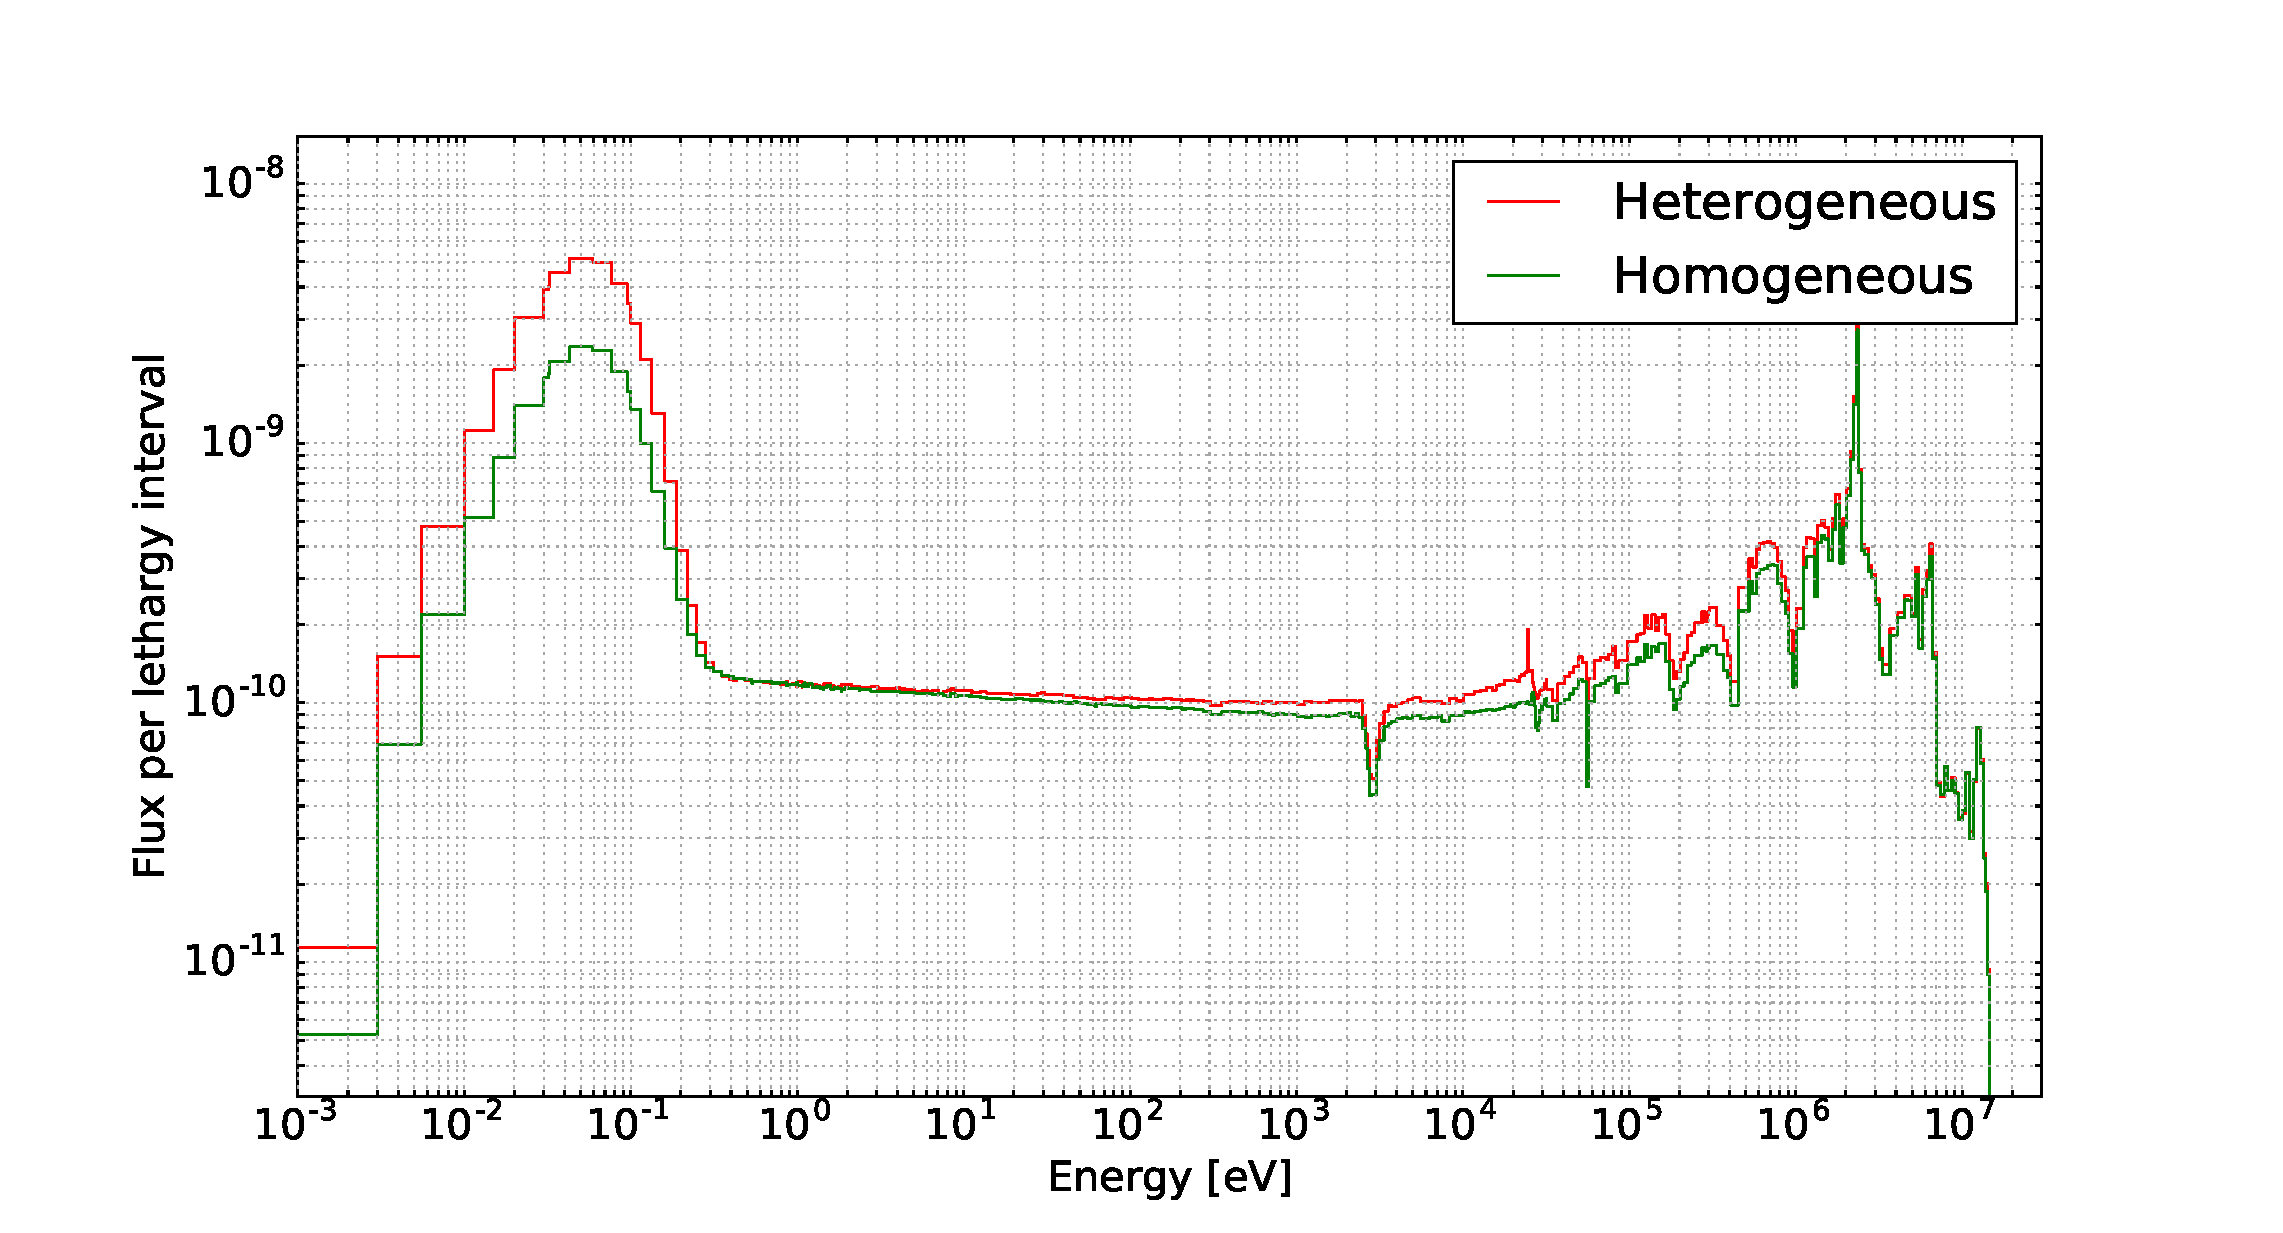
\includegraphics[width=0.9\textwidth]{transmitted_neutron_spectra}
  \caption{The neutron spectra leaving the shield for the heterogeneous and homogeneously modelled cases. This example is for the thickest wall simulated, at 2.1m thickness. The rebar is 41mm in diameter at 200mm spacing, resulting in a steel mass fraction of 4.45\% of the shield total. Note the substantially reduced thermal flux in the homogeneous simulation. The spectrum has been binned with the TRIPOLI 315 group structure.}
  \label{fig:trans_neutron_spec}
\end{figure}

The reduced transmitted homogeneous thermal flux in figure~\ref{fig:trans_neutron_spec} is in part because steel is now available for neutron interactions throughout the depth of the wall, in the homogenised material, rather than solely being available for interactions near the surfaces. Steel has a greater macroscopic material capture cross-section than concrete, and so acts as a neutron sink for slow neutrons, preventing them from propagating through the shield. The material cross-sections for radiative capture are shown in figure~\ref{fig:n_rad_capture}.

\begin{figure}[H]
  \centering
  \figuretitle{Radiative capture probability}
  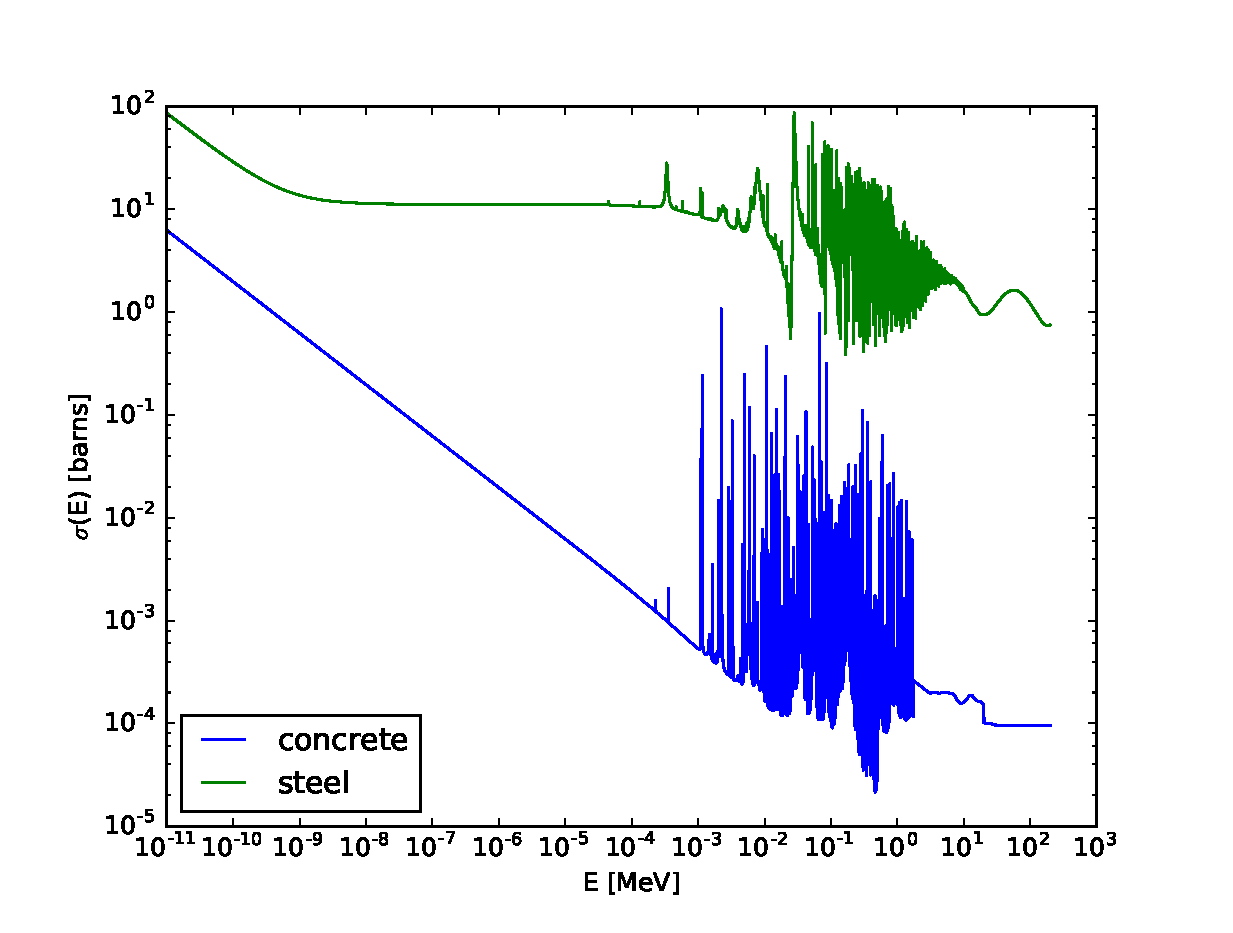
\includegraphics[width=0.8\textwidth]{n_rad_capture}
  \caption{The nuclear properties of steel and concrete are substantially different. Shown here is the cross-section for $(n,\gamma)$ in both materials. At thermal energies steel has a material radiative capture cross-section two orders of magnitude greater than concrete.}
  \label{fig:n_rad_capture}
\end{figure}

Plotting the ratio of the leakage neutron spectra as figure~\ref{fig:relative_neutron_spectra}, one can see the differences in flux more easily. Thermal flux is underestimated by more than a factor 2. But also, fast flux in the 1 keV--1 MeV range is underestimated by $\sim1.2$. The fast flux discrepancy is correlated with wall thickness and is negligible for thin (\textless 1m) walls.

\begin{figure}[H]
  \centering
  \figuretitle{Relative neutron spectra}
  \includegraphics[width=0.8\textwidth]{25HB200_800_relative_n_spectra}
  \caption{The homogeneous flux decreases are readily visible in this figure, principally in the thermal region, but also in the 1 keV -- 1 MeV range. The ratio is of the two spectra from figure~\ref{fig:trans_neutron_spec}. MCNP statistical errors have been combined in quadrature and are plotted as the light shading surrounding the mean value.}
  \label{fig:relative_neutron_spectra}
\end{figure}

Figure~\ref{fig:dose_discrepancy} shows how the received dose discrepancy (as received by someone stood behind the wall) due to the homogeneous approximation varies with wall thickness. Thin walls have a relatively small discrepancy--to be expected as the heterogeneous model is at its most similar to the homogeneous in this case. As the walls become thicker and the rebar meshes become separated by a larger volume of concrete, the discrepancy increases. It plateaus at $\sim 1m$ wall thickness. Similar behaviour is observed for dose due to prompt photons. It can be seen that the effect is greatest for neutrons, with a maximum dose underestimate of 22\%. The great majority of steel in the heterogeneous simulations is orientated perpendicular to the incident neutron flux, although a small number of `stirrup' bars to run parallel with the flux. \citeauthor{Pampin2007} studied water and steel radiation shields, where the orientation of water pipes was varied. Where the pipes were parallel to the incident neutron flux, the spatial homogenisation underestimate was as much as 375\%, as the homogeneous model missed neutron streaming effects \cite{Pampin2007}. However, for the perpendicular configuration as is modelled here, \citeauthor{Pampin2007} found the difference was 13\%, not too dissimilar to the 22\% underestimate reported in this work.

\begin{figure}[H]
  \centering
  \includegraphics[width=0.7\textwidth]{wall_thickness}
  \caption{This figure shows the relationship between the wall thickness and the difference between the homogeneous and heterogeneously modelled walls. The quantity plotted is the energy integrated dose for each case, for neutrons and prompt photons. Error bars due to radiation transport statistics are shown but may not be visible on this scale. The discrepancy between modelling approaches is a function of the wall thickness, greater for neutrons than photons.}
  \label{fig:dose_discrepancy}
\end{figure}

The effect of the steel mass fraction has also been investigated. It was found that the discrepancy between homogeneous and heterogeneous approaches is effectively zero for transmitted photon flux. However, the homogeneous method underestimates neutron flux to a greater degree with an increased steel mass fraction. The greater availability of steel nuclides through the homogeneous mixture results in greater absorption inside the wall and thus a reduced leakage flux (and therefore dose due to neutrons).

% \begin{figure}[H]
%   \centering
%   \figuretitle{Flux ratio at incident surface}
%   \includegraphics[width=0.9\textwidth]{flux_ratio.png}
%   \caption{This visualisation shows the ratio of homogeneous to heterogeneous flux, i.e. the overestimate (> 1) or underestimate (< 1) of neutron flux compared with the true, heterogeneous case. It is a plan view of the reinforced concrete shielding at the side which is first struck by the neutron flux. The reinforcing steel mesh is clearly visible as the area where the homogeneous approximation has raised the flux over its real value.}
%   \label{fig:flux_ratio}
% \end{figure}

\FloatBarrier
\subsection{Shut Down Dose Rate (SDDR)}
\label{subsec:sddr}
After operation of a tokamak, repairs and maintenance are often necessary. This section explores the shut-down dose due to be received from the wall itself. It assumes a worker is inside the bioshield at ITER during a shutdown, stood 30cm from the inner surface of a 150cm thick wall with a steel mass fraction of 4.5\% the total wall mass. Reinforcing bar forms a mesh of squares 20cm in width and height at the front and back of the wall, 5cm from the surfaces. Dose rates due to neutron activation in the reinforced concrete shielding have been calculated for when the reinforced conrete is homogenised and when it is modelled faithfully.

The effect of the spatial homogenisation modelling approximation generally acts to overestimate the SDDR by a small amount. The behaviour is shown as figure~\ref{fig:sddr}. On the timescale of seconds and minutes, and from days out to decades, the overestimate is approximately 10\%. On the timescale of hours, the discrepancy between homogeneous and heterogeneous approaches closes, briefly becoming reversed, with the homogeneous approximation underestimating the SDDR by 4\%. The absolute dose due to photons from the reinforced wall will have fallen by an order of magnitude in the period elapsed between a minute and a week after the final DT shot and it is unlikely anyone will be entering the facility before then.

\begin{figure}[H]
  \centering
  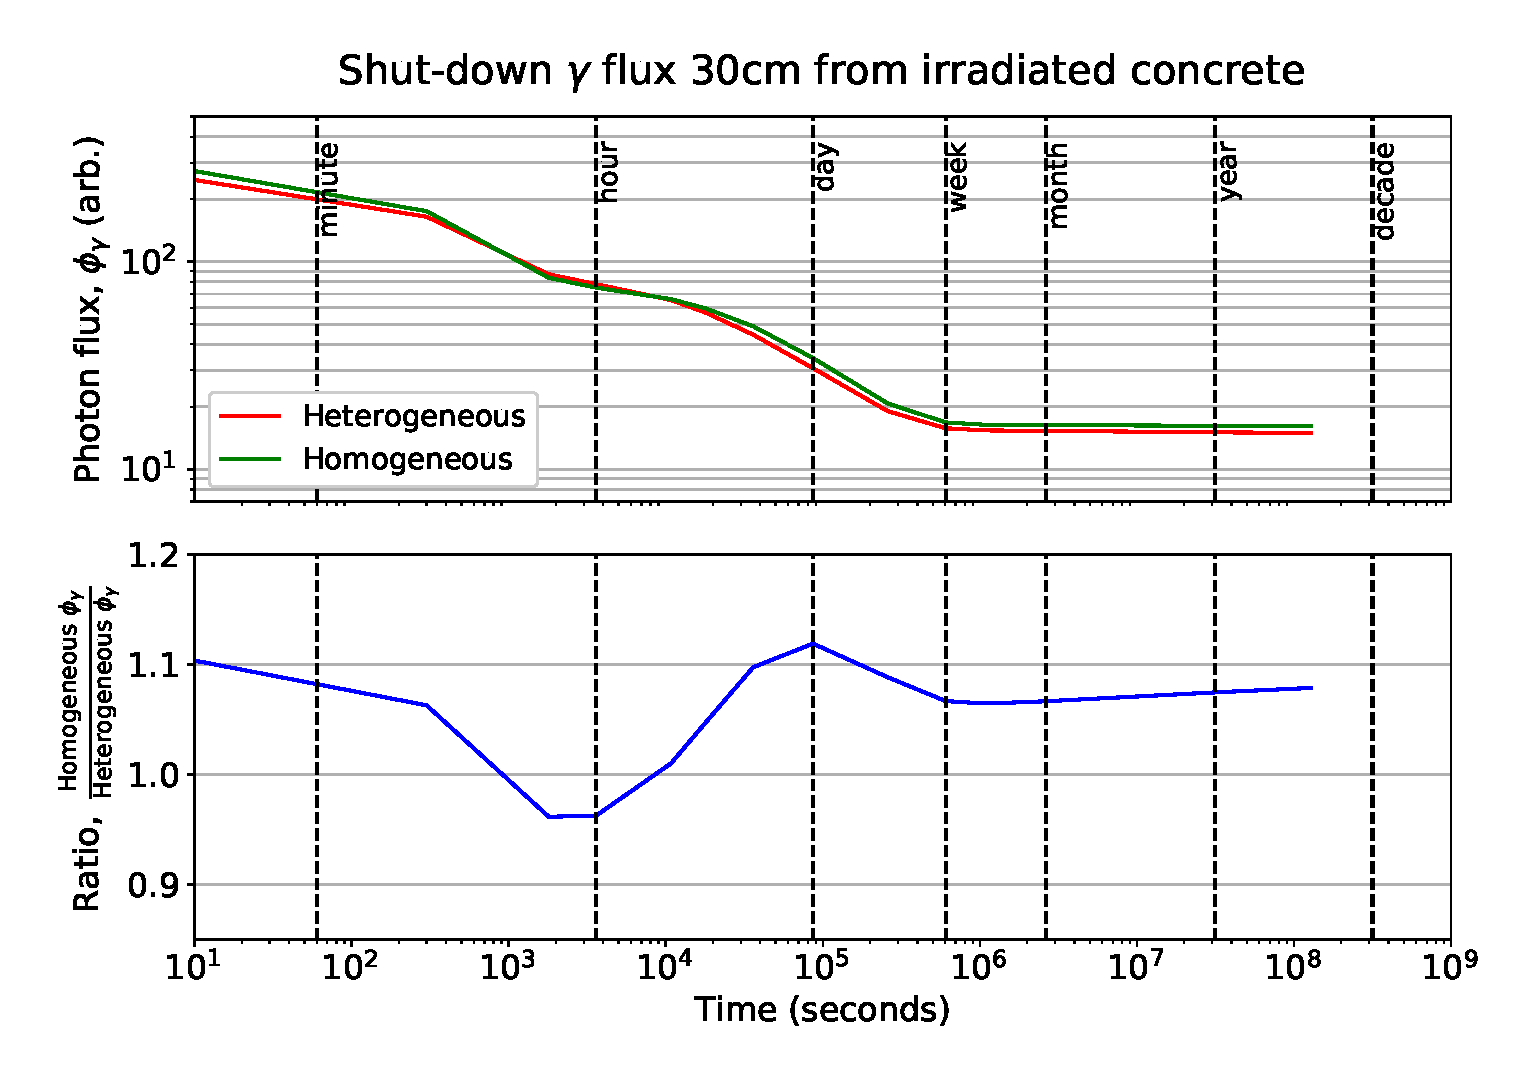
\includegraphics[width=0.8\textwidth]{sddr}
  \caption{This figure displays total $\phi_{\gamma}$ received at a distance of 30cm from the activated wall. The upper panel displays the absolute values in the heterogeneous and homogeneous modelling approaches, as a function of time since last irradiation. There are 16 time steps, for which the activation and subsequent photon transport has been carried out. The lower panel displays the ratio between the approaches, i.e. homogeneous values normalised by the heterogeneous values. One can see that the homogeneous approximation artificially increases the SDDR by $\approx 10\%$ at most time steps, bar those around an hour.}
  \label{fig:sddr}
\end{figure}

The complex behaviour displayed in figure~\ref{fig:sddr} is a result of the many different nuclides which contribute to the decay $\gamma$ field. These nuclides have a range of half-lives and inspecting their relative emissions as a function of time is instructive in understanding the shape of figure~\ref{fig:sddr}. The plot shown as figure~\ref{fig:contact_dose} displays estimates for a contact dose with concrete and steel. As in the real case the reinforcing steel is buried within concrete, the numbers plotted here are not a substitute for transporting decay $\gamma$ photons from their emission to their absorption (as was done for figures~\ref{fig:sddr} \& \ref{fig:sddr_nrg}). Figure~\ref{fig:contact_dose} reports specific contact dose rates, i.e. per unit mass. Note that 2.25\% of the wall mass is steel close to the activated surface, while the mass of concrete between this reinforcing steel and the wall surface is $\frac{5cm}{150cm} (1 - 0.045) = 3.18\%$ of the total wall mass--so the amount of each material near the surface is very roughly equal and therefore specific contact dose rates are informative by themselves, without being weighted by mass.

\begin{figure}[H]
  \centering
  \figuretitle{Contact dose rate by material}
  \includegraphics[width=0.8\textwidth]{contact_dose_by_mat}
  \caption{This plot shows an estimate for the specific contact dose rate due to steel and concrete irradiated under the ITER SA-2 scenario. The total specific dose rate is given by the line plots, with an uncertainty band from EAF-2010 data included as the grey shading. Nuclides which contribute a significant fraction of the dose are shown with their abscissa value as their half-life, $t_{\frac{1}{2}}$ and their ordinate as their contribution to the specific dose rate. The specific dose rate behaviour is quite complex; the material with the highest specific activity changes three times in the simulation period due to various decays.}
  \label{fig:contact_dose}
\end{figure}

From figure~\ref{fig:contact_dose} it is clear that the two materials have quite different nuclear properties, so it is not surprising that their spatial distribution influences the dose received. On a per-mass basis, concrete is more active on the timescale of minutes due to $^{28}$Al, and as this decays the homogeneous overestimate reduces. Subsequently, until a few hours have elapsed since last irradiation, gamma emission from $^{56}$Mn makes steel the most active while the homogeneous approximation begins to overestimate SDDR again. After this, $^{24}$Na in concrete is the dominant contributor to SDDR, making concrete the most active material on the timescale of days. After its decay, the homogeneous approximation falls slightly again as steel becomes the more active material out to very long timescales. 

\begin{figure}[H]
  \centering
  \includegraphics[width=0.8\textwidth]{sddr_nrg.pdf}
  \caption{This figure displays the ratio of homogeneous and heterogeneous $\phi_{\gamma}$ for a series of cooling times and all photon emission energies. Time since last irradiation is given in seconds on the abscissa, while the ordinate is photon emission energy in MeV. The grey circles indicate simulation data, i.e. flux ratios for a particular photon energy group at a particular cooling timestep. These data have been interpolated with the Clough Tocher method to generate the heatmap shown. A diverging colourmap helps identify where spatial homogenisation is overestimating dose (blue) and where it underestimates (red).}
  \label{fig:sddr_nrg}
\end{figure}

Homogeneous simulations tend to overestimate the number of high-energy gamma photons, as can be seen in figure~\ref{fig:sddr_nrg}. A homogeneous overestimate is shown as a blue band across much of the higher energy region. For the homogeneous case, some steel material is located everywhere in the material mixture, including the shallow `cover depth' volume, outside of where the rebar is located in the heterogeneous models. Nuclides from steel then lie on the surface in the homogeneous model and will emit high-energy, gamma rays which can leave the shielding unattenuated and are more likely to contribute to a worker's dose\footnote{High energy gamma-rays (between 1 and 2 MeV) constitute the majority of the dose received at all times, however beyond 2 MeV the flux and therefore contribution to dose falls off sharply.}. Work to corroborate this explanation could include varying the cover depth, to see if homogeneous models started to underestimate the received dose as the cover depth approached zero and the rebar was on the surface in the heterogeneous model.

It is worth noting that while not explicitly modelled here, it is likely that the SDDR on the exterior side of the shield will be artificially depressed by spatial homogenisation as the activating neutron flux is depressed by that approach. This is confirmed for similar circumstances in work by \citeauthor{Sanz2014} \cite{Sanz2014}.

% Sanz is also relevant for cover depth and effects on homogeneous discrepancy -- although requires reinterpretation as the layout is different

\FloatBarrier
\section{Conclusion}
A series of simulations have been performed to assess the impact of the spatial homogenisation modelling approximation on various fluxes and associated doses. 

The specific circumstances investigated are firstly prompt neutron and photon emission from the the ITER plasma and its surroundings, transmitted through a variety of different thickness reinforced concrete walls. In this case, spatial homogenisation was found to underestimate received dose on the outside of the wall by up to 22\%, with the discrepancy a function of wall thickness. For photons, there was less effect, with 10\% the greatest divergence between approaches. The relatively small discrepancies are to be expected for reinforcing bar arrangements as used here. 

The second case investigated how spatial homogenisation affected the dose to workers during a maintenance operation, the SDDR at the inside face of a wall activated by neutron irradiation. This particular configuration is relatively unaffected by spatial homogenisation, with the greatest deviation from the true case being an overestimate of 12\% for the homogenised case. The discrepancy is a function of the cooling time, with a smaller discrepancy at timescales beyond a day, down to an overestimate of approximately 8\%. As the homogenised results are dose overestimates, they are in this case conservative, and thus do not pose a risk to workers' health, rather providing an upper bound on the likely dose rate. 

Where the practice of spatial homogenisation likely results in a conservative estimate as is the case here, it can be tolerated, as it reduces model complexity and is safe. However, where neutron streaming paths are available, if features contain routes with low absorption or poor moderating properties, or if features are larger than the mean free path of the neutrons, then spatial homogeisation should be treated with caution. One imagines that with the increased computer power available for nuclear and multi-physics analysis, in the not distant future details such as reinforcing bar and other small but potentially important features will be explicitly included in radiation transport models. 

% Comment on size of these uncertainties relative to hydrogen fraction (water content) \cite{Samarin2013} and concrete density 
% pg12 Pampin2007 useful for general guidance on spatial homogenisation

